\chapter{Reinforcement Learning}\label{reinforcement_learning}
% hier könnte noch was sinnvolles stehen
% https://github.com/Unity-Technologies/ml-agents/blob/master/docs/Background-Machine-Learning.md
Das vorherige Kapitel \ref{intelligente_agenten} beschäftigt sich mit der Entwicklung intelligenter Agenten zur Erschaffung von künstlicher Intelligenz für virtuelle Entitäten in Videospielen. Der Fokus dieses Kapitels liegt in der Erläuterung von Reinforcement Learning (RiL) als eine alternative Methode. Die Nutzung von Machine Learning stellt den logischen nächsten Schritt zu den bereits vorgestellten Methoden für die Realisierung \textit{lernender} intelligenter Agenten in Videospielen dar. Im Gegensatz zu klassischen Methoden werden hier also Agenten verwendet, die aufgrund ihrer gesammelten Erfahrungen einen Lernprozess durchlaufen. Das Kapitel dient als vorbereitendes Element für die Implementierung von lernenden intelligenten Agenten in einem Dorfsystem als zentrales Thema der vorliegenden Thesis.

Insgesamt wird ein starker Fokus auf \ac{reinforcement_learning} gesetzt. Zunächst wird dafür eine Gegenüberstellung zwischen klassischen Machine Learning-Verfahren und \ac{reinforcement_learning} vorgenommen. Es folgt eine Einordnung der Verfahren in einen übergeordneten Kontext sowie die Beschreibung aktueller Entwicklungen in diesem Bereich. Anschließend werden \acp{markov_problem} als elementare Problemstellung für \ac{reinforcement_learning} diskutiert. Ein Menge konkreter modellfreier und modellbasierter Methoden zur Implementierung des Verfahrens werden ausführlich erläutert. Dafür werden nötige mathematische Grundlagen geschaffen.

Der erste Abschnitt beinhaltet eine Rekapitulation zur grundsätzlichen Funktionsweise von \Fachbegriff{Machine Learning}. Zur Einordnung des Themas in einen übergeordneten Kontext findet anschließend eine Einordnung der klassischen Teilbereiche von Machine Learning und \ac{reinforcement_learning} statt. 




\section{Einordnung}
Maschinelles Lernen beschäftigt sich mit der Entwicklung eines Systems, das aus einer Menge von beliebigen Inputdaten einen gewünschten Output erzeugt. Dabei wird der Versuch unternommen, durch eine Verbesserung des Outputs in Abhängigkeit vom Input einen Lerneffekt zu erzielen. Diese Fähigkeit wird erlangt, indem das System mit relevanten Informationen gespeist wird, aus denen Assoziationen gebildet und Muster erkannt werden können. Dadurch können schlussendlich zukünftige Outputs verbessert werden, ohne dass dieser Vorgang spezifisch definiert wird. Der Lernvorgang passiert nicht durch die Nutzung eines statischen Algorithmus und wird nicht explizit programmiert, sondern wird durch die automatische Anpassung von Werten und Gewichtungen beschrieben, die dem System zugrunde liegen. Häufig werden hierfür neuronale Netze verwendet. Man entscheidet dabei unter anderem zwischen \Fachbegriff{Feedforward}-Netzen und \Fachbegriff{rekurrenten} Netzen. Feedforward-Netze verbinden stets Neuronen aus vorderen Schichten mit Neuronen aus hinteren Schichten. Rekurrente neuronale Netze erlauben auch umgekehrte Verbindungn von vorderen Neuronen zu hinteren Neuronen. So entsteht eine Rückkopplung, die zeitliche Informationen aus zuvor getätigten Entscheidungen mit einbeziehen kann.
Ein System, das einen Input manipuliert, wird also so lange verändert, bis es für jeden Output den gewünschten Input erzeugen kann. Anstatt Beispiele auswendig zu lernen wird ein statistisches Modell erzeugt, das auch unbekannte Daten beurteilen kann. Dieses Modell wir durch eine Menge von Parametern beschrieben, in der Regel handelt es sich dabei um die Gewichtungen der einzelnen Neuronen in einem neuronalen Netz.

Weiterhin sollte geklärt werden, was als Input und als Output für das System genutzt wird. Wir gehen im Folgenden davon aus, dass ein einfaches neuronales Netz verwendet wird, dessen Struktur für die Lösung des folgenden Problems irrelevant ist. Um den Lernvorgang eines Agenten zu ermöglichen, müssen für den Input Werte gewählt werden, die für die Problemstellung relevant sind. Dabei kann es sich um beliebige Informationen aus dem Weltzustand des Spiels handeln. Im Folgenden wird ein Beispiel betrachtet, das indirekt bereits das Vorgehen beim \ac{reinforcement_learning} beschreibt, um das generelle Vorgehen von maschinellem Lernen zu verdeutlichen.

Ein Agent soll lernen, auf einer sich bewegenden Plattform zu balancieren. Für diese Aufgabe gibt es bestimmte relevante Parameter - beispielsweise die Orientierung der Plattform sowie die Orientierung des Agenten. Unter der Annahme, dass keine weiteren äußeren Parameter die Problemstellung beeinflussen, werden diese beiden Vektoren als Inputparameter für das neuronale Netz verwendet. Zusätzlich muss definiert werden, was die Outputparameter des neuronalen Netzes steuern sollen. In diesem simplen Szenario ist es offensichtlich, dass für das Balancieren die Orientierung des Agenten angepasst werden muss.
Nun findet ein Lernvorgang statt, indem durch eine kontinuierliche Änderung der Strategie des Agenten durch die Anpassung seines Modells Beziehungen zwischen Input und Output hergestellt werden können. Der Agent sammelt \Fachbegriff{Erfahrungen}, indem er über einen langen Zeitraum versucht, das Problem zu lösen und währenddessen immer wieder von der Plattform fällt. Einige Entscheidungen führen jedoch dazu, dass der Agent sich länger auf der Plattform halten kann als andere. Es werden Assoziationen zwischen der Orientierung der Plattform und des Agenten sowie dem Erfolg der jeweils gesammelten Erfahrungen gebildet. Das Modell des Agenten bzw. dessen Strategie als Reaktion auf die Inputparameter wird kontinuierlich angepasst, bis der Agent das Balancieren beherrscht.
Man spricht hier vom \textit{Training} eines neuronalen Netzes. Der Trainingsvorgang unterscheidet sich dabei je nach verwendeter Technologie. Es wird weiterhin zwischen \Fachbegriff{Training} und \Fachbegriff{Inference} unterschieden. Die Inference beschreibt die Nutzung eines bereits trainierten Machine Learning-Modells zur Generierung eines Outputs. Dabei werden im Unterschied zum Training keine Gewichtungen mehr angepasst. Das fertige Modell wird nicht verändert, sondern lediglich genutzt.
Generell unterscheidet man zwischen einem überwachten Training mithilfe von bereits bekannten Inputdaten, denen ein bekannter Output zugeordnet wurde oder einem unüberwachten Training, für das derartige Daten nicht vorhanden sind. Weiterhin wird in der vorliegenden Arbeit \ac{reinforcement_learning} als zusätzliche Kategorie angeführt. Im Folgenden werden zunächst unüberwachte und überwachte Methoden näher betrachtetet.

% vorteile, nachteile von ML (geld sparen und besseren content erzeugen)?
% die problematik und den ablauf besser erklären


\subsection{Überwachtes Lernen}\label{supervised_learning}
Das \Fachbegriff{überwachte Lernen} (\Fachbegriff{supervised learning}) basiert auf der Verwendung von Trainingsdaten, die über bestimmte \Fachbegriff{Label} verfügen. Diese Label sind Werte oder Einordnungen in Klassen, die ein bestimmtes Beispiel aus dem Datensatz beschreiben und über die jedes Beispiel des Datensatzes verfügen muss. Beispielsweise könnte es sich um eine Menge von Bildern von Pflanzen handeln, wobei jedes Bild mit dem Namen der Pflanze versehen ist. Diese Klassifizierungen sind bereits vor dem Trainingsvorgang bekannt. Es ist weiterhin genau bekannt, was der Output des Verfahrens ist, nämlich eine Klassifizierung der Beispiele in Klassen von Pflanzen.
Häufig wird diese Methode daher für Klassifizierungsaufgaben verwendet. Dabei müssen allgemeine Muster, Gemeinsamkeiten und Unterschiede zwischen den Beispielen identifiziert werden, sodass das Verfahren aus den gefundenen Merkmalen lernt, Label aus Bildinformationen vorherzusagen. Anders formuliert ist der Input in das neuronale Netz eine Menge von Bildinformationen, der Output ist jeweils ein Label bzw. eine Klasse.
Zusätzlich kann überwachtes Lernen für Regressionen verwendet werden. Es gilt, folgende Frage zu beantworten: \glqq{}Wenn eine Variable $x$ einen bestimmten Wert hat, welchen Wert hat dann $y$?\grqq{}. Ein mögliches Anwendungsszenario wäre ein neuronales Netz, das den Preis einer Wohnung in Hamburg anhand ihrer Lage, Ausstattung und Größe bestimmt.

\subsubsection{Imitation Learning}\label{imitation_learning}
Bei \Fachbegriff{Imitation Learning} (\Fachbegriff{Imitation Learning}) handelt es sich um eine Kombination aus \ac{reinforcement_learning} und überwachtem Lernen, bei der bereits vorhandene Daten verwendet werden, um Sequenzen von zukünftigen Aktionen vorherzusagen \cite{icml_imitation}. Imitation Learning wird häufig in Spielen verwendet um intelligente Agenten zu erschaffen die versuchen, die Aktionen eines Spielers zu imitieren. Man spricht auch von \Fachbegriff{Behavioral Cloning}. Als Trainingsdaten können beispielsweise Aufzeichnungen des Spielverhaltens eines echten Spielers dienen. Sowohl die Beobachtungen aus dem Spielzustand als auch die daraus resultierenden Entscheidungen des Spielers anhand seines Hardwareinputs sind gegeben, um eine Imitation zu ermöglichen. Gegeben sind also sowohl Beobachtungen, als auch die resultierenden Aktionen; nun muss der Zusammenhang zwischen den Beiden gelernt werden. In der Rennspielreihe \Fachbegriff{Forza Motorsport} wurde Imitation Learning erfolgreich eingesetzt, um sogenannte \sogenannt{Drivatars} \cite{forza} zu erstellen. Dabei handelt es sich um Agenten, die genau das Fahrverhalten von spezifischen Spielern imitieren sollen.


\subsection{Unüberwachtes Lernen}\label{unsupervised_learning}
Trainingsdatensätze sind nicht für jedes Machine Learning-Problem gegeben. Tatsächlich ist das Fehlen von gelabelten Daten häufig ein Problem, da das Anfertigen solcher Datenmengen eine lange Zeit in Anspruch nehmen würde oder in bestimmten Szenarien gar nicht möglich ist.
Beim \Fachbegriff{unüberwachten Lernen} bekommt ein neuronales Netz während des Trainingsvorgangs eine Menge von nicht gelabelten Daten ohne spezielle Anweisungen. Anhand von Labeln ist es hier also nicht möglich, bestimmte Merkmale in den Trainingsdaten zu erkennen. Stattdessen werden alternative Ansätze gewählt, zum Beispiel:
\begin{itemize}
    \item \texttt{Clustering}: Bestimmte Charakteristiken oder \Fachbegriff{Features} werden aus den Daten extrahiert. Dabei kann es sich im oben genannten Pflanzenbeispiel um die Größe der Blätter, Farbe der Blüten oder die Form handeln. Die Beispiele werden anhand von Ähnlichkeiten angeordnet, also \sogenannt{geclustered}.
    \item \texttt{Anomaly Detection}: Anomalien in den Features werden erkannt, um \sogenannt{Ausreißer} zu erkennen. Wenn beispielsweise alle Pflanzen im Datensatz gelbe Blüten haben außer Eine, so würde Diese als Anomalie erkannt werden.

Im Gegensatz zum überwachten Lernen ist der Output des Modells unbekannt. Weiß man beispielsweise beim überwachten Lernen genau, dass als Output eine Klassifizierung der Beispiele in eine bestimmte Anzahl von Pflanzenkategorien vorgenommen wird, so muss beim unüberwachten Lernen der Output genau analysiert werden, um ein Verständnis darüber zu erlangen. Es ist weiterhin vorher nicht immer klar, wie viele Kategorien bzw. Cluster gebildet werden und wie die Verteilung der Beispiele aussieht.
Durch das Fehlen von Referenzdaten ist eine Überprüfung der Genauigkeit des Verfahrens beim unüberwachten Lernen oft schwierig.
\end{itemize}


\subsection{Reinforcement Learning}\label{reinforcement_learning_intro}
Der Begriff \Fachbegriff{Reinforcement Learning} beschreibt ein Verfahren, in dem ein Agent eigenständig lernt, sinnvolle Entscheidungen zu treffen, indem aus einer Menge von Aktionen diejenigen ausgewählt werden, die eine Belohnungsfunktion maximieren \cite{ai_for_game_devs} \cite{reinforcement_introduction_book} \cite{dammann_reinforcement} \cite{alzantot_0} \cite{intel_ai_demystifying}. Zur Anwendung kommt es neben Videospielen ebenfalls in der Robotik oder in der Medizin. Der grundsätzliche Ablauf von \ac{reinforcement_learning} wird in Abbildung \ref{fig:reinforcement_flow} dargestellt.

\begin{figure}[H]
\centering
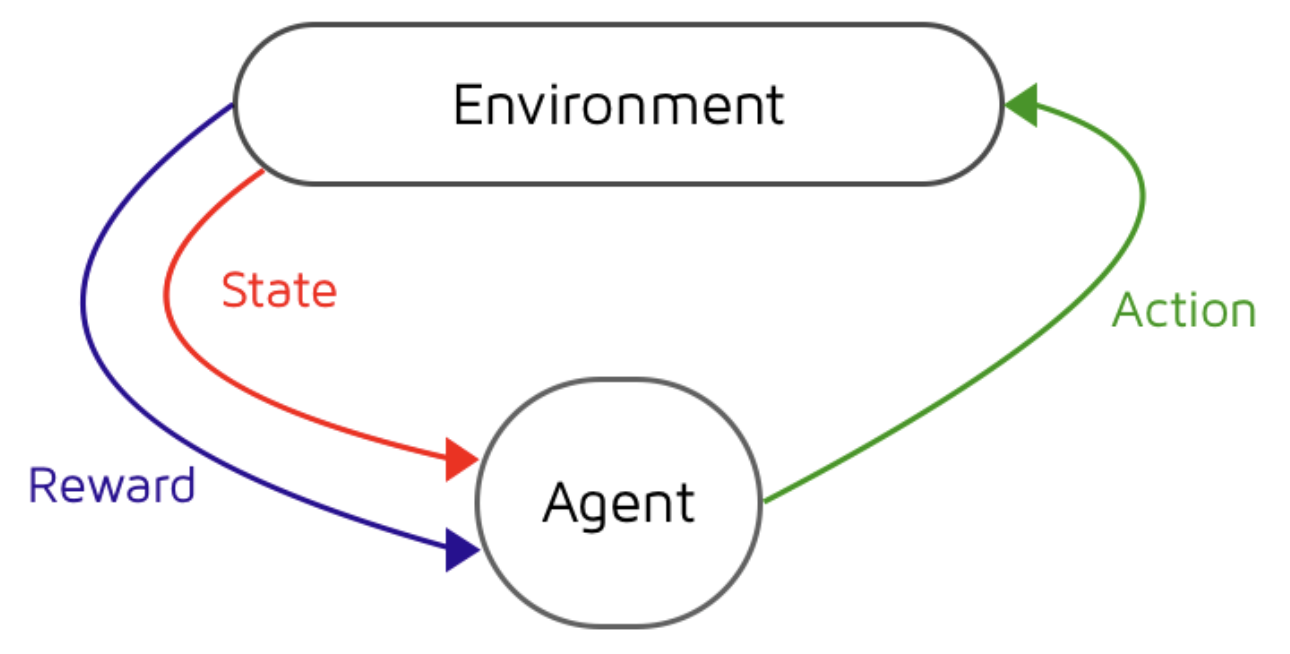
\includegraphics[scale=0.45]{images/reinforcement_flow.png}
\caption{Grundsätzlicher Ablauf von \ac{reinforcement_learning} \cite{intel_reinforcement_openai_gym_blog}}
\label{fig:reinforcement_flow}
\end{figure}

Die Ausführung einer Aktion versetzen den Agenten in einen neuen Zustand und resultiert in einer Belohnung (\Fachbegriff{Reward}) oder einer Bestrafung (\Fachbegriff{Punishment}). Es handelt sich um einen skalaren Wert, der beschreibt, wie gut der Agent sich verhalten hat. Der Zustand des Agenten wird durch Beobachtungen (\Fachbegriff{Observations}) aus seiner Umgebung (\Fachbegriff{Environment}) beschrieben. Der Agent soll aus seinen Erfahrungen lernen, indem er die besten Aktionen wählt, die die zukünftige Summe seiner Belohnungen maximieren. Der Lernvorgang erfolgt dabei durch die kontinuierliche Änderung seiner Entscheidungsstragie in Abhängigkeit von seinem Zustand, indem beispielsweise Gewichtungen in einem zugrunde liegenden neuronalen Netz angepasst werden. Dabei wird der Versuch unternommen, die Belohnungsfunktion zu maximieren, indem die Beziehungen zwischen Beobachtungen und gewählten Aktionen, sowie den jeweils resultierenden Belohnungen modelliert werden. Für die Suche der besten Entscheidung werden zusätzlich zukünftige Belohnungen berechnet und mit einbezogen (siehe \Fachbegriff{Markov Decision Problems} in Abschnitt \ref{markov_decision_problems}). Generell muss nicht explizit ein klares Ziel definiert werden, stattdessen führt das eigenständige Lernen dazu, dass sich das optimale Verhalten eines Agenten automatisiert ergibt.


Eine Kategorisierung von \ac{reinforcement_learning} in \Fachbegriff{überwachtes Lernen} oder {unüberwachtes Lernen} (siehe Abschnitte \ref{supervised_learning} und \ref{unsupervised_learning}) ist schwierig. Im Gegensatz zum unüberwachten Lernen können den möglichen Aktionen konkrete Werte zugewiesen werden, die das Verhalten des Agenten bewerten. Anstelle des Aufspürens von Anomalien oder Clustern wird also versucht, dem Verhalten des Agenten einen Wert bzw. ein \textit{Label} zuzuweisen. Im Unterschied zum überwachten Lernen werden hier allerdings keine gelabelten Trainingsdatensätze verwendet, sondern eine Menge von Belohnungswerten die sich erst zur Zeit des Trainingsvorgangs ergeben. Bei der Entscheidungsfindung sind beim Reinforcement Learning zudem nicht nur einzelne Vorhersagen relevant, sondern ganze Sequenzen. Man kann also weder von überwachtem, noch von unüberwachtem Lernen sprechen. \ac{reinforcement_learning} wird daher als eine zusätzliche Kategorie betrachtet, die sich von den genannten klassischen Verfahren abgrenzt und eine Art Hybrid-Verfahren darstellt.

Für die Entwicklung intelligenter Agenten ist unüberwachtes Lernen im klassischen Sinne nicht geeignet, da dort mit der Extrahierung markanter Features und Zusammenhänge in Datensätzen ein gänzlich anderes Ziel verfolgt wird. Wegen fehlender gelabelter Datensätze eignet sich auch überwachtes Lernen nicht. Man stelle sich ein Szenario vor, in dem ein Agent das Schachspielen lernen soll: Für eine große Menge von denkbaren Situationen würden dann Daten mit dem jeweiligen Label für den korrekten auszuwählenden Zug benötigt. Diese große Datenmenge müsste mühselig angefertigt bzw. gesammelt werden. Im deterministischen Falle von Schach wäre das Sammeln dieser Daten beispielsweise durch die Aufzeichnung von Spielen in einer Schachapp möglich. Diese Möglichkeit ist jedoch nicht mehr gegeben, sobald das Zielverhalten des Agenten unbekannt ist oder die Umgebung nicht-deterministische Strukturen aufweist.
\ac{reinforcement_learning} bietet hingegen ein leicht zu handhabendes Framework, in dem Probleme auf eine simple Art und Weise beschrieben werden können. In der Theorie müssen hier lediglich gute Züge positiv und schlechte Züge negativ bewertet werden, sodass der Agent aus den Belohnungen in Kombination mit seinen Beobachtungen Schlüsse ziehen kann. Weiterhin fällt die Notwendigkeit von großen (gelabelten) Datensätzen weg.
Aktuelle Projekte (siehe Kapitel \ref{aktuelle_entwicklungen_rl}) zeigen dabei vielversprechende Ergebnisse und beweisen sowohl die Skalierbarkeit als auch das hohe Lernpotential von \ac{reinforcement_learning}-basierten Algorithmen. Mit Projekten wie \Fachbegriff{OpenAI Gym} \cite{openai_gym} und \Fachbegriff{ML-Agents} \cite{ml-agents_paper} (siehe Abschnitt \ref{ml_unity}) stehen darüber hinaus umfangreiche Umgebungen und Bibliotheken für die Einbindung in Spiele bereit. Weiterhin finden sich keine vergleichbaren Ansätze in der Fachliteratur, die auf \ac{reinforcement_learning} zur Definition des Verhaltens von \acp{npc} setzen, wodurch ein Gegenpol zu klassischen Verfahren gesetzt und eine neuartige Methode getestet werden kann.

\ac{reinforcement_learning} bietet aus den genannten Gründen den sinnvollsten und möglichweise einzigen realistischen Lösungsansatz für das gebotene Problem und wird daher in der vorliegenden Arbeit verwendet.




















\section{Markov Decision Problems}\label{markov_decision_problems}
Dieses Kapitel beschäftigt sich mit der Erläuterung von \acp{markov_problem} als Grundlage für das \Fachbegriff{Reinforcement Learning}, welches die Lösung von \Fachbegriff{Markov-Problemen} anstrebt. Daher bilden sie eine wichtige Basis für das folgende Kapitel. 
Bei Markov-Problemen (bzw. \Fachbegriff{Markov-Entscheidungsproblemen}) handelt es sich um ein Modell für Entscheidungsprobleme, bei denen ein Agent versucht, eine Belohnungsfunktion zu maximieren \cite{ai_for_game_devs} \cite{reinforcement_introduction_book} \cite{deep_reinforcement_paper} \cite{art_int_mod_app} \cite{dammann_reinforcement} \cite{alzantot} \cite{mohammad_markov}. Zu jeder Entscheidung befindet sich der Agent in einem bestimmten Zustand und verfügt über eine Menge von Aktionen, aus denen er wählen kann. Durch die Ausführung von Aktionen bewirkt der Agent Übergänge in andere Zustände. Es muss einen oder mehrere Endzustände geben, die die Ausführung abbrechen, sobald sie erreicht werden. Die Wahrscheinlichkeit für die Auswahl einer Aktion liegt jeweils bei einem Wert von $p < 1$.
Wenn ein Agent stets die beste Entscheidung trifft, dann spricht man von einer optimalen \Fachbegriff{Policy} für die Lösung des Problems. Eine Policy ist also eine Strategie des Agenten in Abhängigkeit von seinem Zustand, welcher durch Beobachtungen aus seiner Umgebung festgelegt wird. Diese werden auch \Fachbegriff{Observations} genannt. Die Policy kann weiterhin definiert werden als eine Funktion vom Zustand eines Agenten zu einer Wahrscheinlichkeitsverteilung über die möglichen Aktionen \cite{openai_five_paper}.

\subsection{Beispiel}
Im folgenden Beispiel wird ein Roboter betrachtet \cite{markov_robot_example}, der sich jeweils um ein Feld in vier Richtungen bewegen kann. Wenn dieser die Wände des in Abbildung \ref{fig:markov_problem_1} sichtbaren Spielfelds berührt, dreht er automatisch um und bewegt sich in die gegenüberliegende Richtung. Nur die weißen Felder sind passierbar. Felder, die mit einer Zahl versehen sind, geben Belohnungen oder Bestrafungen. Hier wird ein skalarer Wert $+1$ oder $-1$ genutzt. Das Feld mit einer Bestrafung heißt \Fachbegriff{Bestrafungsfeld}. Weitere Felder resultieren jeweils in einer Bestrafung von $-0.04$. Das Ziel ist es, den besten Weg zum Ziel (dem Feld mit der \textit{+1}) mit der höchsten Belohnung für den Roboter zu finden.

\begin{figure}[H]
\centering
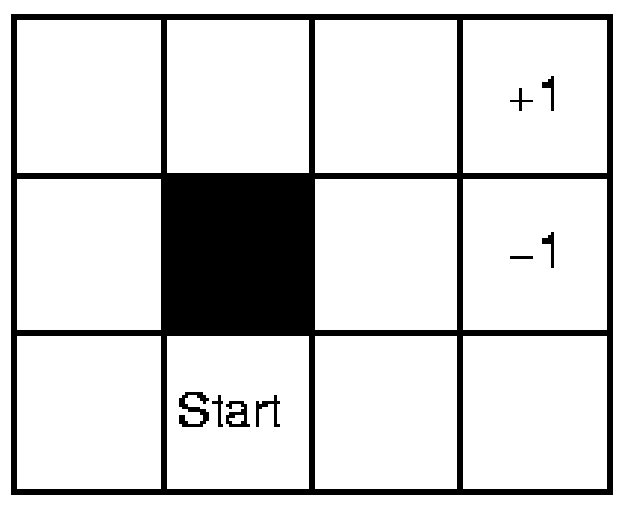
\includegraphics[scale=0.4]{images/markov/markov_problem_1.png}
\caption{Deterministisches MDP \cite{markov_robot_example}}
\label{fig:markov_problem_1}
\end{figure}

Betrachtet wird nun ein deterministischer Ansatz. Hier gehen wir davon aus, dass der Roboter die Aktionen, die er auswählt, immer korrekt ausführt. Als bester Weg ergibt sich dabei mathematisch der kürzeste Weg, wie in Abbildung \ref{fig:markov_problem_2} zu sehen. Da das Szenario leicht in einen Graphen mit Kosten transformiert werden kann, ist offensichtlich, dass Suchverfahren wie A* verwendet werden können, um den optimalen Pfad zu finden.

\begin{figure}[H]
\centering
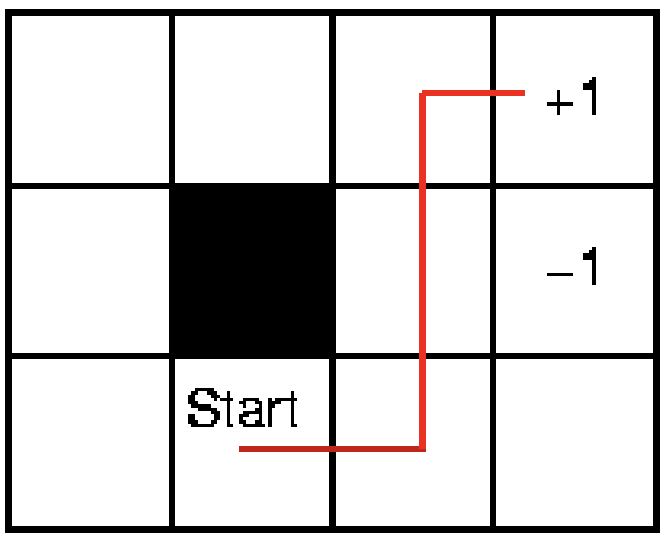
\includegraphics[scale=0.39]{images/markov/markov_problem_2.png}
\caption{Lösung des deterministischen MDP \cite{markov_robot_example}}
\label{fig:markov_problem_2}
\end{figure}

Nun wird ein nichtdeterministischer bzw. stochastischer Ansatz gewählt. Bei solchen Problemen spricht man von einem \ac{pomdp}. Die Zustandsübergänge bekommen dann einen stochastischen Wert zugewiesen. Das bedeutet, dass der Roboter Aktionen nun mit einer gewissen Wahrscheinlichkeit korrekt oder inkorrekt ausführen kann. Die Umgebung des Agenten ist also nichtdeterministisch.

Die Wahrscheinlichkeiten für das Roboter-Beispiel sind in Abbildung \ref{fig:markov_problem_3} erkennbar. Der Agent hat in seiner Laufrichtung eine Chance von $p = 0,8$ und zu den Seiten hin jeweils eine Wahrscheinlichkeit von $p = 0,1$. Das bedeutet, dass der Agent nur in 80\% der Fälle die gewünschte Aktion und in 20\% der Fälle die falsche Aktionen ausführt.

\begin{figure}[H]
\centering
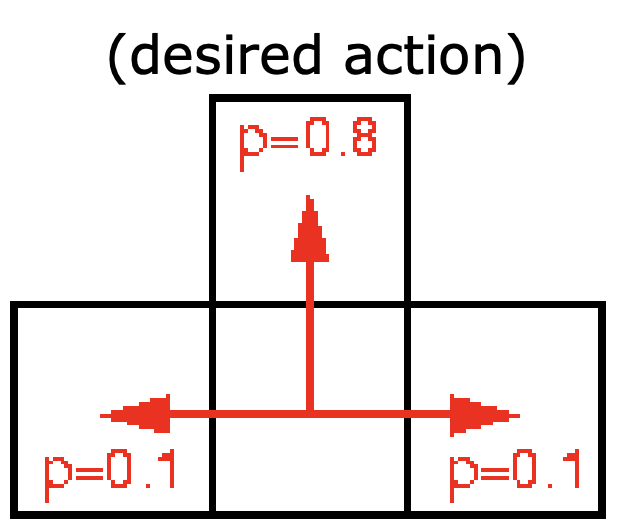
\includegraphics[scale=0.34]{images/markov/markov_problem_3.png}
\caption{Nichtdeterministisches MDP \cite{markov_robot_example}}
\label{fig:markov_problem_3}
\end{figure}

\begin{figure}[H]
\centering
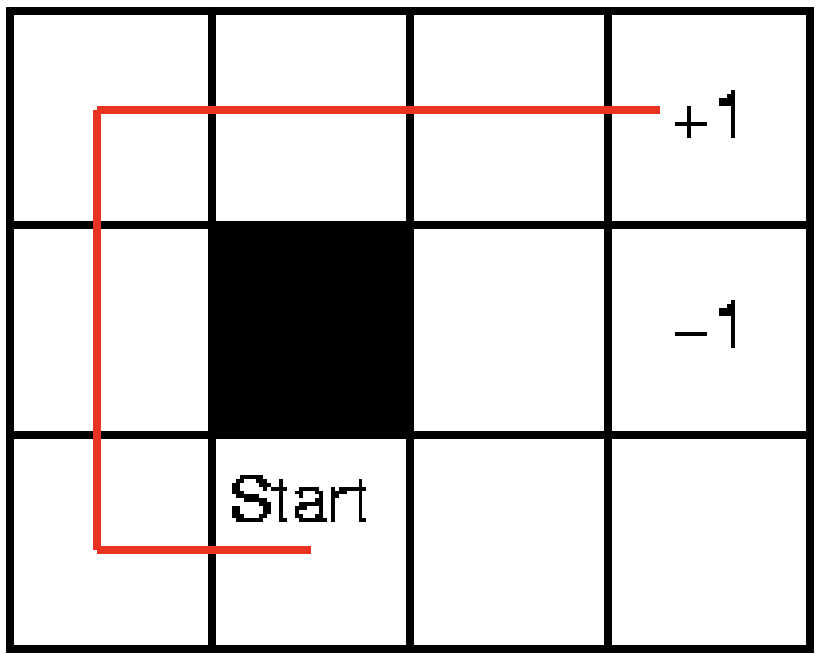
\includegraphics[scale=0.32]{images/markov/markov_problem_4.png}
\caption{Lösung des nichtdeterministischen MDP \cite{markov_robot_example}}
\label{fig:markov_problem_4}
\end{figure}

Abbildung \ref{fig:markov_problem_4} zeigt den resultierenden besten Weg. Anstatt den kürzesten Weg zu wählen wird nun ein Weg gewählt, bei dem die Wahrscheinlichkeit geringer ist, durch eine falsch ausgeführte Aktion versehentlich das Bestrafungsfeld zu betreten. Statistisch gesehen ergibt sich daraus die höchste Belohnung für den Agenten. In diesem Fall kann das Problem also nicht ohne Weiteres durch einen Suchalgorithmus gelöst werden, da es nichtdeterministisch ist.



\subsection{Formale Beschreibung}
Nachdem im vorherigen Kapitel zum Verständnis je ein Beispiel für ein deterministisches \ac{markov_problem} und ein nichtdeterministisches \ac{markov_problem} geliefert wurde, folgt in diesem Abschnitt eine formale Beschreibung von Markov-Problemen.


Sei $N$ ein Agent in einer Umgebung $\epsilon$ mit einer Anzahl diskreter Zeitschritte $t$. Die Umgebung kann beispielsweise durch eine virtuelle Welt in einem Spiel dargestellt werden. $N$ verfügt über endlich viele Zuständen $s_t$ aus der Menge aller möglichen Zustände $\mathbb{S}$ mit einer jeweils dazugehörigen Aktion $a_t$. Die jeweils nächsten Zustände heißen $s_t+1$ und $a_t+1$. Zu jedem Zeitschritt $t$ wählt $N$ durch $\pi$ eine neue Aktion $a_t$ aus einer endlichen Menge von Aktionen $\mathbb{A}$. Der Agent $N$ erhält nach $a_t$ einen neuen Zustand $s_t+1$ und eine Belohnung $r_t$. Dieser Prozess wiederholt sich, bis ein  Terminalzustand $s_t$ erreicht wurde.

$N$ verfügt über eine Policy $\pi$. Diese wurde bereits definiert als eine Funktion, die den aktuellen Zustand $s_t$ aus $\mathbb{S}$ nimmt und eine Aktion $a_t$ aus $\mathbb{A}$ zurückgibt. Formal wird $\pi$ also wie folgt beschrieben:
$$ \pi(s_t) : \mathbb{S} \rightarrow \mathbb{A} $$

Aus den einzelnen Belohnungen ergibt sich dann eine akkumulierte Gesamtbelohnung $R_t$, wobei gilt:
$$   R_t   =   \sum_{k=0}^{\infty} {\gamma^k * r_{t+k}}   $$

Die Summe von $0$ bis $\infty$ wird gebildet, weil davon ausgegangen wird, dass es kein Zeit- bzw. Zeitschrittlimit gibt. In der oben sichtbaren Definition beschreibt $\gamma$ den sogenannten \Fachbegriff{Discount-Faktor}. Er wird wie folgt definiert:
$$ \gamma \in \interval[open left]{0}{1} $$

Nach jeder ausgeführten Aktion werden alle Belohnungen, die der Agent theoretisch noch erreichen kann, mit $\gamma$ multipliziert. Dies führt dazu, dass weiter in der Zukunft liegende Belohnungen eine geringere Gewichtung bekommen. Eine weit entfernte hohe Belohnung kann durch die Gewichtung des Discount-Faktors eine deutlich kleinere tatsächliche Belohnung darstellen und damit für den Agenten \sogenannt{uninteressant} werden. Der optimale Lösungsweg wird durch einen Discount-Faktor $\gamma < 1$ so  verändert, dass der Agent im Allgemeinen kürzere Wege bevorzugt. Zu kleine Werte führen dazu, dass der Agent keine langfristigen Belohnungen berücksichtigen kann und kurzsichtige Entscheidungen trifft.

Das Ziel des Agenten ist also die Maximierung der gesamten zukünftigen Belohnung, also der Gesamtbelohnung $R_t$ für jeden Zustand $s_t$. Die potentielle Belohnung wird durch die gewichtete Summe der erwarteten Belohnungswerte für alle zukünftigen Aktionen gebildet, wobei alle möglichen Aktionen in Betracht gezogen werden. Dadurch wird effektiv die aktuell auszuwählende Aktion durch zukünftige Belohnungen beeinflusst.

Es wurde ein Beispiel für Markov-Probleme demonstriert und eine formale Beschreibung aufgestellt. Der nächste Schritt besteht nun in der Lösung von Markov-Problemen. Als weitere Voraussetzung wird im Folgenden kurz die \Fachbegriff{Markov-Eigenschaft} erläutert.



\subsection{Markov-Eigenschaft}
Es wird ein Szenario betrachtet, in dem ein Agent die Zustände $A$, $B$, $C$ und $D$ annehmen kann \cite{markov_property_example}. Die Wahrscheinlichkeit für das sequentielle Auftreten der genannten Zustände hintereinander kann wie folgt faktorisiert werden:

$$ p(A,B,C,D) = p(A) p(B|A) p(C|A,B) p(D|A,B,C)   \;\; $$
$$ \;\;\;\;\;\;\;\;\;\;\;\;\;\;\;\;\;\;\;\;\;\;\;\;\; = p(B) p(A|B) p(C|A,B) p(D|A,B,C)   \;\; ... $$
$$ \;\;\;\;\;\;\;\;\;\;\;\;\;\;\;\;\;\;\;\;\;\;\;\;\; = p(C) p(A|C) p(B|A,C) p(D|A,B,C)   \;\; ... $$
$$ \;\; ... $$

Die \Fachbegriff{Markov-Eigenschaft} gilt, wenn es eine ausgezeichnete (z.B zeitliche) Anordnung gibt, für die sich die Darstellung wie folgt vereinfachen lässt \cite{markov_property_example}:

$$ p(A,B,C,D)  = p(A) p(B|A) p(C|B) p(D|C) $$

Das bedeutet, dass die Wahrscheinlichkeit für den nächsten Zustand nur unmittelbar von dem vorherigen Zustand abhängt. Die Wahrscheinlichkeit für $C$ hängt also nur vom vorherigen $B$ und nicht von dem ursprünglichen $A$ ab.